    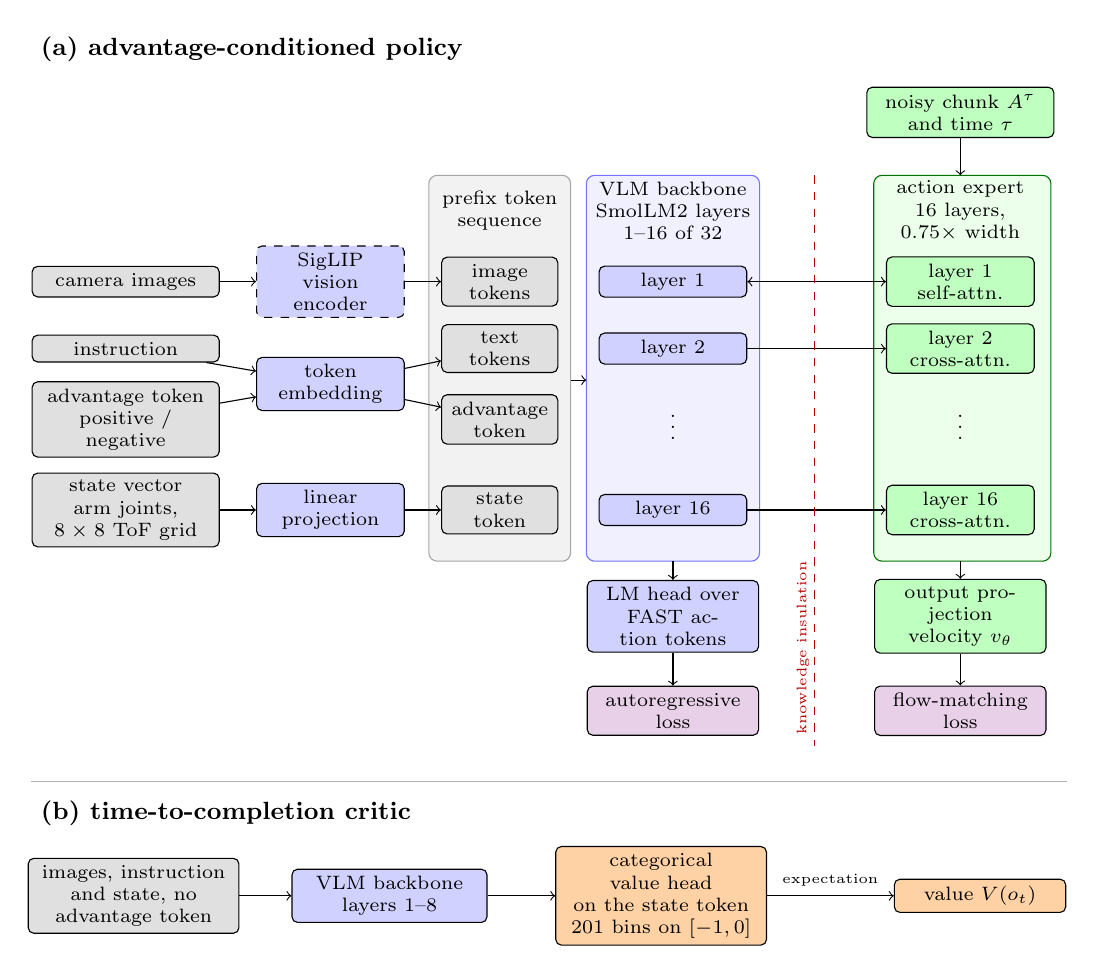
\begin{tikzpicture}[
        font=\scriptsize,
        blk/.style={draw, rounded corners=2pt, align=center, inner sep=2.5pt},
        data/.style={blk, fill=black!12},
        vlm/.style={blk, fill=blue!18},
        exp/.style={blk, fill=green!25},
        loss/.style={blk, fill=violet!18},
        crit/.style={blk, fill=orange!35}]

    % ---------- panel (a): the policy ----------
    \node[anchor=west, font=\small\bfseries] at (0,2.95) {(a) advantage-conditioned policy};

    \draw[draw=black!35, fill=black!5, rounded corners=3pt] (5.05,1.35) rectangle (6.85,-3.55);
    \draw[draw=blue!55, fill=blue!6, rounded corners=3pt] (7.05,1.35) rectangle (9.25,-3.55);
    \draw[draw=green!45!black, fill=green!8, rounded corners=3pt] (10.70,1.35) rectangle (12.95,-3.55);

    \node[align=center] at (5.95,0.90) {prefix token\\sequence};
    \node[align=center] at (8.15,0.90) {VLM backbone\\SmolLM2 layers\\1--16 of 32};
    \node[align=center] at (11.80,0.90) {action expert\\16 layers,\\0.75$\times$ width};

    \node[data, text width=2.2cm] (img) at (1.20,0.00) {camera images};
    \node[data, text width=2.2cm] (instr) at (1.20,-0.85) {instruction};
    \node[data, text width=2.2cm] (adv) at (1.20,-1.75) {advantage token\\positive / negative};
    \node[data, text width=2.2cm] (st) at (1.20,-2.90) {state vector\\arm joints, $8\times8$ ToF grid};

    \node[vlm, dashed, text width=1.7cm] (siglip) at (3.80,0.00) {SigLIP\\vision encoder};
    \node[vlm, text width=1.7cm] (temb) at (3.80,-1.30) {token\\embedding};
    \node[vlm, text width=1.7cm] (sproj) at (3.80,-2.90) {linear\\projection};

    \node[data, text width=1.3cm] (p1) at (5.95,0.00) {image tokens};
    \node[data, text width=1.3cm] (p2) at (5.95,-0.85) {text tokens};
    \node[data, text width=1.3cm] (p3) at (5.95,-1.75) {advantage token};
    \node[data, text width=1.3cm] (p4) at (5.95,-2.90) {state token};

    \node[vlm, text width=1.7cm] (v1) at (8.15,0.00) {layer 1};
    \node[vlm, text width=1.7cm] (v2) at (8.15,-0.85) {layer 2};
    \node at (8.15,-1.75) {$\vdots$};
    \node[vlm, text width=1.7cm] (v16) at (8.15,-2.90) {layer 16};

    \node[exp, text width=1.7cm] (e1) at (11.80,0.00) {layer 1\\self-attn.};
    \node[exp, text width=1.7cm] (e2) at (11.80,-0.85) {layer 2\\cross-attn.};
    \node at (11.80,-1.75) {$\vdots$};
    \node[exp, text width=1.7cm] (e16) at (11.80,-2.90) {layer 16\\cross-attn.};

    \node[exp, text width=2.2cm] (noisy) at (11.80,2.15) {noisy chunk $A^\tau$\\and time $\tau$};

    \node[vlm, text width=2.0cm] (lmhead) at (8.15,-4.25) {LM head over\\FAST action tokens};
    \node[loss, text width=2.0cm] (arloss) at (8.15,-5.45) {autoregressive\\loss};
    \node[exp, text width=2.0cm] (outproj) at (11.80,-4.25) {output projection\\velocity $v_\theta$};
    \node[loss, text width=2.0cm] (fmloss) at (11.80,-5.45) {flow-matching\\loss};

    \draw[->] (img) -- (siglip);
    \draw[->] (instr) -- (temb);
    \draw[->] (adv) -- (temb);
    \draw[->] (st) -- (sproj);
    \draw[->] (siglip) -- (p1);
    \draw[->] (temb) -- (p2);
    \draw[->] (temb) -- (p3);
    \draw[->] (sproj) -- (p4);
    \draw[->] (6.85,-1.25) -- (7.05,-1.25);
    \draw[<->] (v1) -- (e1);
    \draw[->] (v2) -- (e2);
    \draw[->] (v16) -- (e16);
    \draw[->] (noisy) -- (11.80,1.35);
    \draw[->] (8.15,-3.55) -- (lmhead);
    \draw[->] (lmhead) -- (arloss);
    \draw[->] (11.80,-3.55) -- (outproj);
    \draw[->] (outproj) -- (fmloss);

    \draw[red!70!black, dashed] (9.95,1.35) -- (9.95,-5.90);
    \node[rotate=90, font=\tiny, text=red!70!black] at (9.80,-4.65) {knowledge insulation};

    % ---------- panel (b): the critic ----------
    \draw[black!30] (0,-6.35) -- (13.15,-6.35);
    \node[anchor=west, font=\small\bfseries] at (0,-6.75) {(b) time-to-completion critic};

    \node[data, text width=2.5cm] (cin) at (1.30,-7.80) {images, instruction and state, no advantage token};
    \node[vlm, text width=2.3cm] (cvlm) at (4.55,-7.80) {VLM backbone\\layers 1--8};
    \node[crit, text width=2.5cm] (chead) at (8.00,-7.80) {categorical value head\\on the state token\\201 bins on $[-1,0]$};
    \node[crit, text width=2.0cm] (cval) at (12.05,-7.80) {value $V(o_t)$};

    \draw[->] (cin) -- (cvlm);
    \draw[->] (cvlm) -- (chead);
    \draw[->] (chead) -- node[above, font=\tiny] {expectation} (cval);
    \end{tikzpicture}
